\begin{boiboiboite}
	\propair
	\isentropiques
	\isothermes
\end{boiboiboite}

% idea: aircraft tyre deflation after MERTO

\subsubsection{Pression d’air}
\label{exo_pression_air}

	Une masse de~\SI{5}{\kilogram} d’air est enclose dans un réservoir de~\SI{2}{\metre\cubed}.

	\begin{enumerate}
		\item Quelles sont son volume spécifique et sa masse volumique ?
		\item Quelle est la pression si la température est de~\SI{20}{\degreeCelsius} ?
	\end{enumerate}
	
\subsubsection{Réchauffement d’un réservoir d’air}
\label{exo_rechauffement_reservoir_air}
\wherefrom{dérivé du rattrapage S1 2013}% reconstruit à partir du rattrapage 20130621

	Un réservoir hermétique d’air comprimé en béton a un volume fixe de~\SI{1,2}{\metre\cubed}. L’air y est stocké à pression de~\SI{2}{\bar}. \\
	Le réservoir est placé au soleil et le réchauffement solaire fait passer la température de~\SI{5}{\degreeCelsius} à~\SI{60}{\degreeCelsius}.
	
	\begin{enumerate}
		\item Quelles sont la masse, le volume spécifique, la masse volumique et la pression à l’intérieur du réservoir, avant et après le réchauffage ?
	\end{enumerate}

	Lorsque la température atteint~\SI{60}{\degreeCelsius}, une soupape s’ouvre et laisse de l’air s’échapper pour faire redescendre la pression dans le réservoir jusqu’à la pression initiale de~\SI{2}{\bar}. Pendant l’échappement, la température de l’air à l’intérieur du réservoir reste constante.

	\begin{enumerate}
		\shift{1}
		\item Quelle masse d’air doit-on laisser échapper ?
	\end{enumerate}

	Lorsque la pression a atteint~\SI{2}{\bar}, la soupape se referme et le réservoir, de nouveau hermétique, se refroidit lentement à volume constant. La température finale revient à~\SI{5}{\degreeCelsius}.
	
	\begin{enumerate}
		\shift{2}
		\item Quelle est la pression finale dans le réservoir ?
	\end{enumerate}


\subsubsection{Énergie et température}
\label{exo_gp_energie_temperature}

	De l’air dans un compartiment flexible est à pression de~\SI{3}{\bar}. Son énergie interne est de~\SI{836}{\kilo\joule\per\kilogram}.
	
	Il est chauffé à pression constante jusqu’à~\SI{900}{\degreeCelsius} ; il est ensuite refroidi et détendu alors que ses propriétés varient selon la relation $p v^{\num{1.1}} = \text{cste.}$ jusqu’à ce que sa température atteigne~\SI{25}{\degreeCelsius}.

	\textit{[Question piège]} Combien d’énergie a-t-il reçu ou perdu depuis le début de l’évolution ?

\subsubsection{Puissance d’une pompe à air}
\label{exo_puissance_pompe_air}

	Une pompe à air (\cref{exo_compresseur_air}) comprime de l’air en régime permanent, de façon adiabatique. L’air voit sa température augmenter de~\SI{15}{\degreeCelsius} à~\SI{100}{\degreeCelsius}.
	
	Quelle est la puissance spécifique consommée ?

	\begin{figure}[!bh]
		\begin{center}
			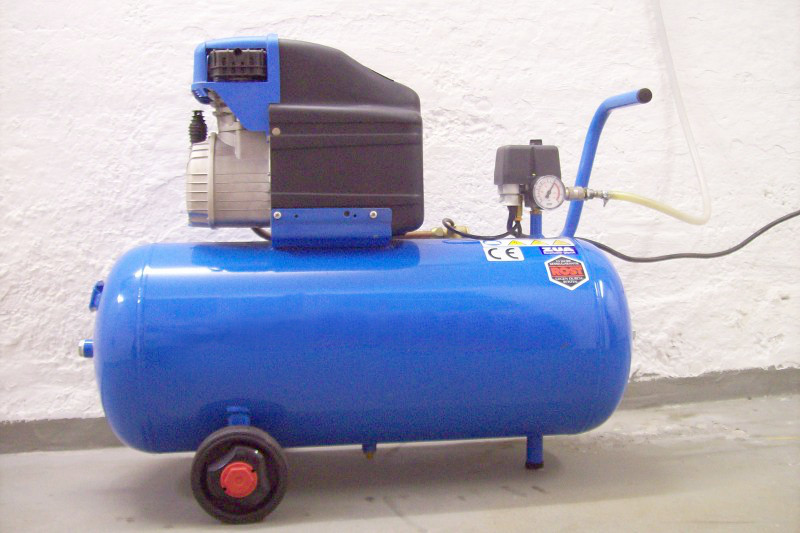
\includegraphics[width=0.6\columnwidth]{images/compresseur_air_reservoir.jpg}
		\end{center}
		\supercaption{Un petit compresseur électrique monté sur un réservoir d’air portatif}{image dérivée \wcfile{Kolbenkompressor.jpg}{d’une photo} \pd par \wcu{Grikalmis}}
		\label{fig_exo_compresseur_air}
	\end{figure}
	
\onlyamphibook{\par~\clearfloats\dontbreakpage}%handmade
\subsubsection{Turbine de turboréacteur}
\label{exo_gp_turbine_turboreacteur}
\wherefrom{[DS n°2 2011, 3pts]}
	
	Un/e étudiant/e démonte le turboréacteur \textit{\wf{Turbomeca Marboré}} d’un \wfd{Fouga CM-170 Magister}{Fouga Magister} pour en étudier et en modifier le fonctionnement. Il/elle fait fonctionner le moteur sur un banc d’essai.
	
	À l’entrée de la turbine, les conditions sont mesurées à~\SI{110}{\metre\per\second} et~\SI{1000 }{\degreeCelsius} .\\
	À la sortie de la turbine, ces propriétés sont mesurées à~\SI{125}{\metre\per\second} et~\SI{650}{\degreeCelsius} .
	
	L’étudiant/e mesure également les pertes sous forme de chaleur de la turbine : \SI{75}{\kilo\joule\per\kilogram}.
	
	\begin{enumerate}
		\item Quelle est la puissance mécanique spécifique développée par la turbine ?
		\item Quelle condition l’étudiant/e doit-il/elle maintenir pour obtenir une puissance de~\SI{1}{\mega\watt} ?
	\end{enumerate}


\subsubsection{Évolutions élémentaires : Compression isotherme}
\label{exo_gp_isotherme}
\wherefrom{[DS n°2 2011, 4pts]}
% Cet exo est lié à l’exercice 8.5 (\ref{exo_diagrammes_ts})

	Une masse de~\SI{3,5}{\kilogram} d’air est comprimée de façon réversible isotherme (à température constante) depuis~\SI{2}{\bar} et~\SI{15}{\degreeCelsius} jusqu’à~\SI{45}{\bar}.
	
	\begin{enumerate}
		\item Représentez l’évolution sur un diagramme pression-volume, de façon qualitative (c’est-à-dire sans représenter les valeurs numériques).
		\item Quelles sont les quantités de travail et de chaleur mises en jeu ?
		\item Si la compression était effectuée de façon adiabatique réversible, le volume final serait-il différent ?
	\end{enumerate}
	

\subsubsection{Évolutions élémentaires : refroidissements isobare et isochore}
\label{exo_gp_isobare_isochore}
\wherefrom{[DS n°2 2010, 5pts]}
% Cet exo est lié à l’exercice 8.5 (\ref{exo_diagrammes_ts})

	Une masse de~\SI{2}{\kilogram} d’air dans un réservoir déformable est à pression de~\SI{4,5}{\bar} et occupe un volume de~\SI{800}{\liter}. Elle est refroidie et le réservoir maintient la pression constante jusqu’à ce que le volume ait été réduit de~\SI{40}{\percent}.
	
	Ensuite, le refroidissement est continué à volume constant jusqu’à ce que la température atteigne~\SI{25}{\degreeCelsius}.
	
	\begin{enumerate}
		\item Tracez l’évolution suivie sur un diagramme pression-volume.
		\item Quel est le travail effectué par l’air ?
		\item Quel est le coût total en chaleur pour la totalité de l’évolution ?
	\end{enumerate}


\subsubsection{Évolutions élémentaires : compression isentropique}
\label{exo_gp_isentropique}
	
	Quelle quantité minimale de travail faut-il pour comprimer~\SI{5}{\kilogram} d’air à~\SI{1}{\bar} et~\SI{20}{\degreeCelsius} jusqu’à \SI{50}{\bar} sans transfert de chaleur ? Tracez l’évolution suivie par l’air sur un diagramme pression-volume.


\subsubsection{Évolutions élémentaires : vocabulaire}
\label{exo_bete_mechant}
\wherefrom{[DS n°2 2010, 2pts]}

	Une masse fixe de gaz parfait, avec pour seul espoir de contrarier un/e étudiant/e en thermodynamique, suit lentement les évolutions suivantes :

		\begin{center}
			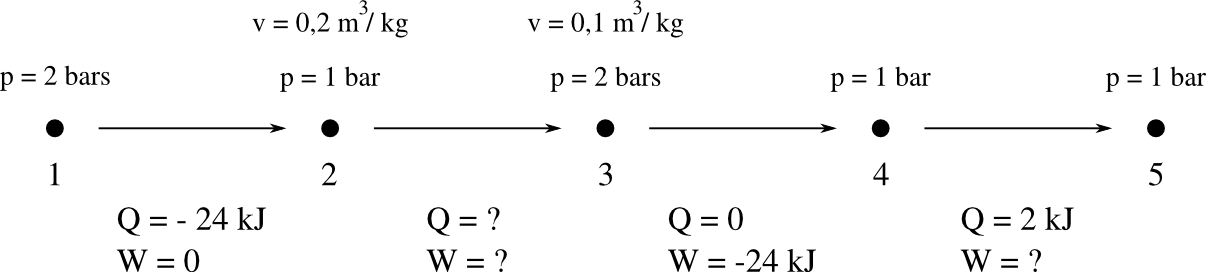
\includegraphics[width=\textwidth]{images/exo_elementaires.png}
		\end{center}

	Parmi les évolutions ci-dessus, lesquelles sont :
	\begin{enumerate}
		\item à température constante (isotherme) ?
		\item à volume constant (isochore) ?
	\end{enumerate}


\subsubsection{Évolutions élémentaires : pression et volume}
\label{exo_retrouver_pv}
\wherefrom{Partiel S1 2013, 2pts}

	Parmi les évolutions réversibles décrites en \cref{fig_pvel}, identifiez (sans vous justifier) l’évolution à température constante, à pression constante, adiabatique réversible, et à volume constant.
	
	\begin{figure}[!bh]
		\begin{center}
			%\vspace{-0.1cm}%handmade
			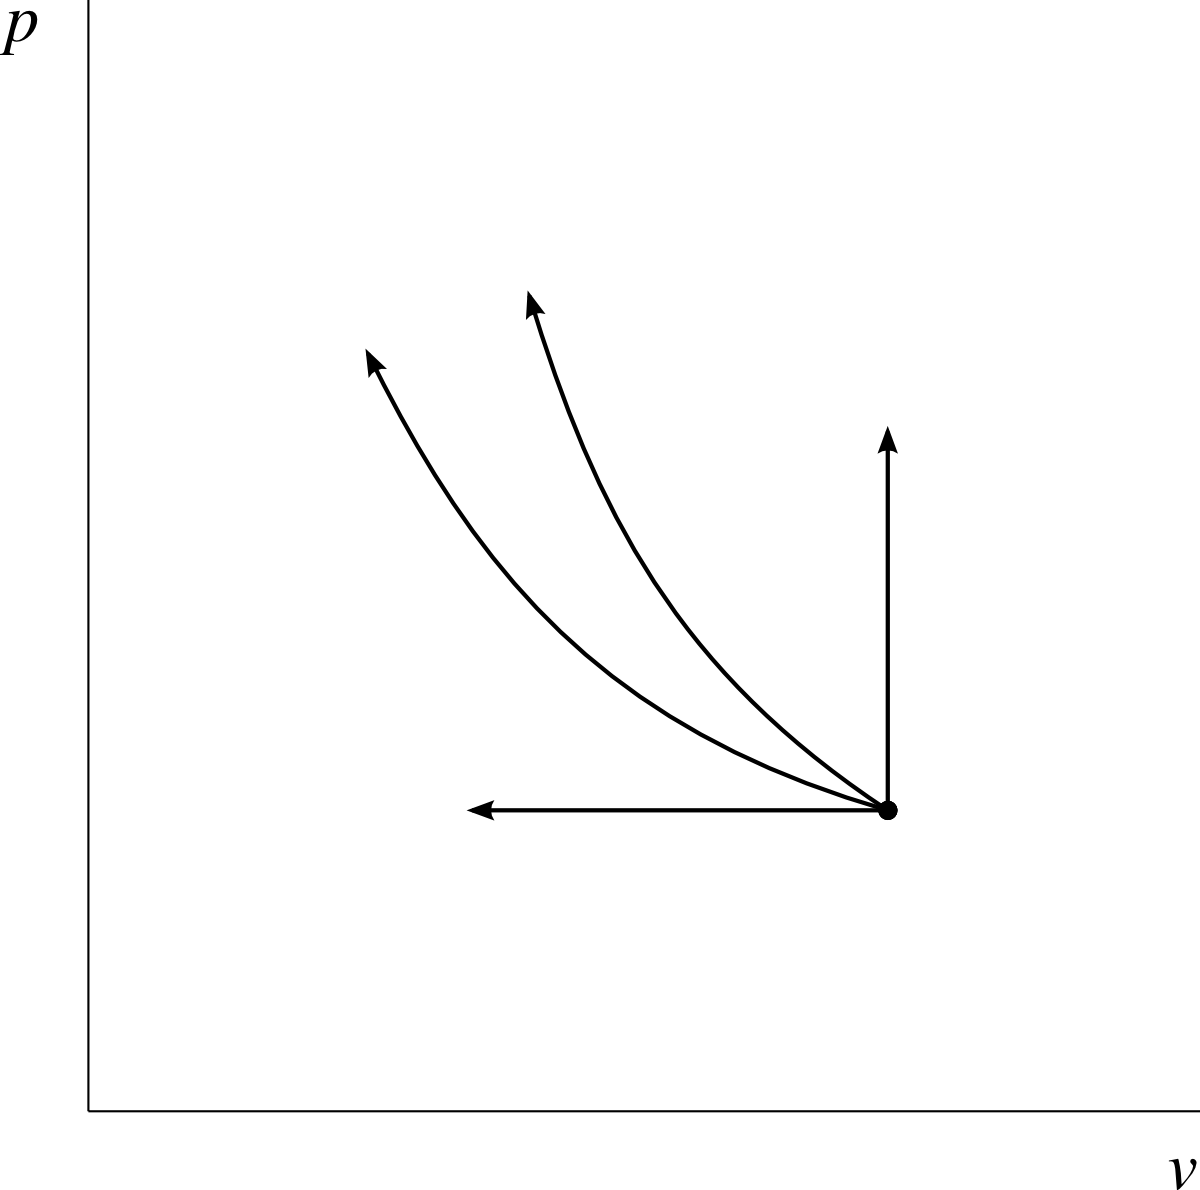
\includegraphics[width=0.4\textwidth, max width=0.6\columnwidth]{images/exo_pv_elementaires1.png}
			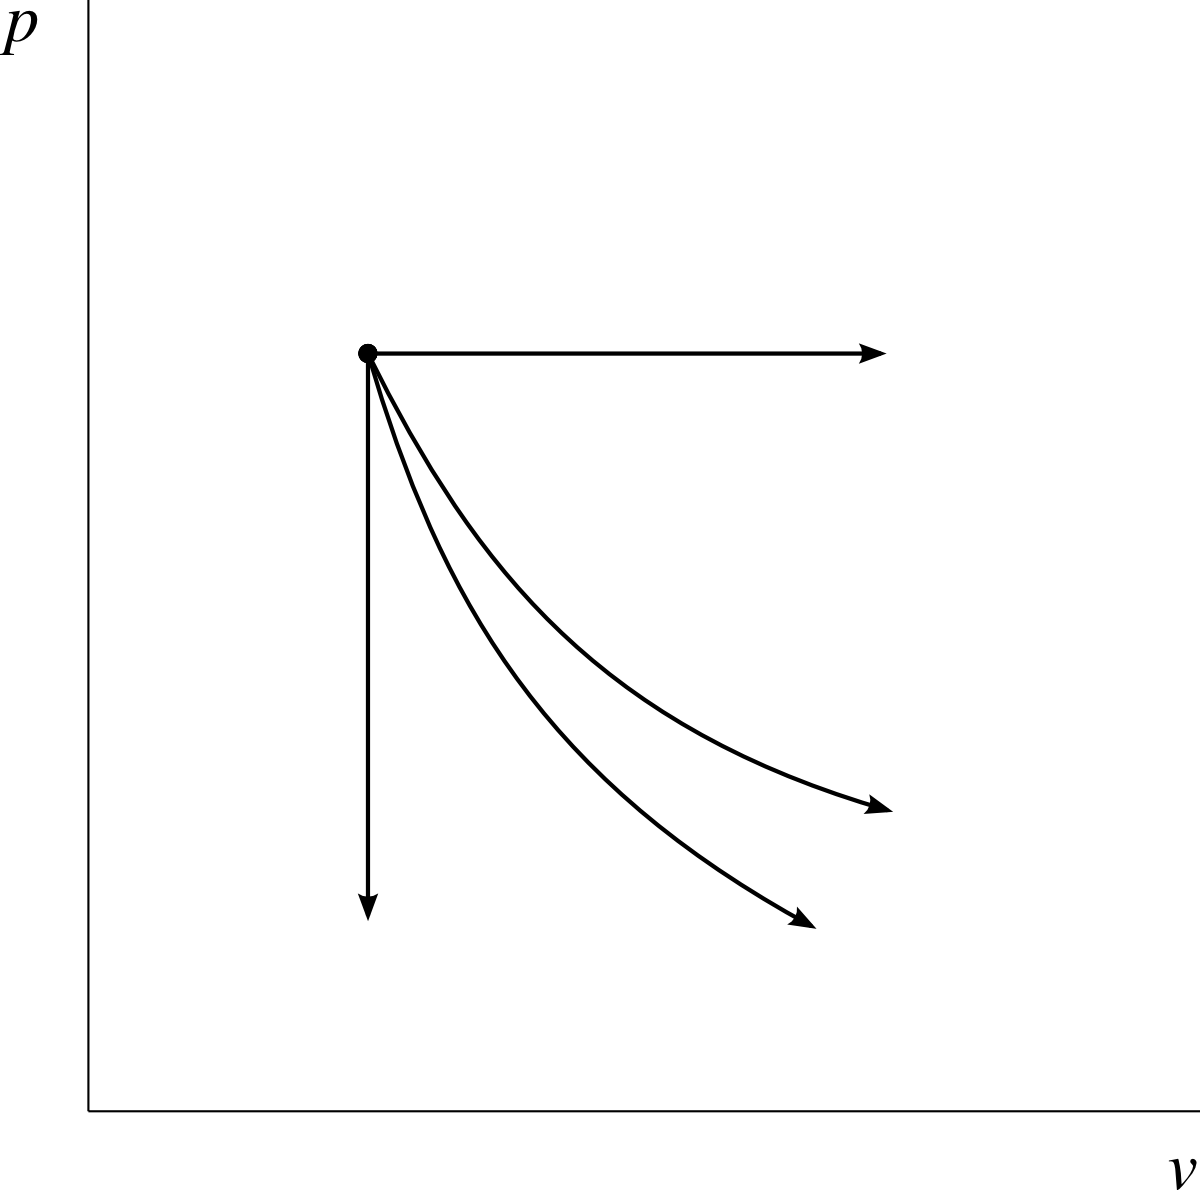
\includegraphics[width=0.4\textwidth, max width=0.6\columnwidth]{images/exo_pv_elementaires2.png}
			%\vspace{-0.1cm}%handmade
		\end{center}
		\supercaption{Évolutions élémentaires d’un gaz parfait}{schéma \cczero \oc}
		\label{fig_pvel}
	\end{figure}
	

\subsubsection{Compresseur de turboréacteur}
\label{exo_compresseur_turboreacteur}
\wherefrom{[Partiel S1 2012, 8pts]}

	À l’intérieur d’un des moteurs d’un avion de ligne, le compresseur (\cref{fig_exo_entree_genx2b}) est quasiment adiabatique.	
	
	\begin{figure}[bh]
		\begin{center}
			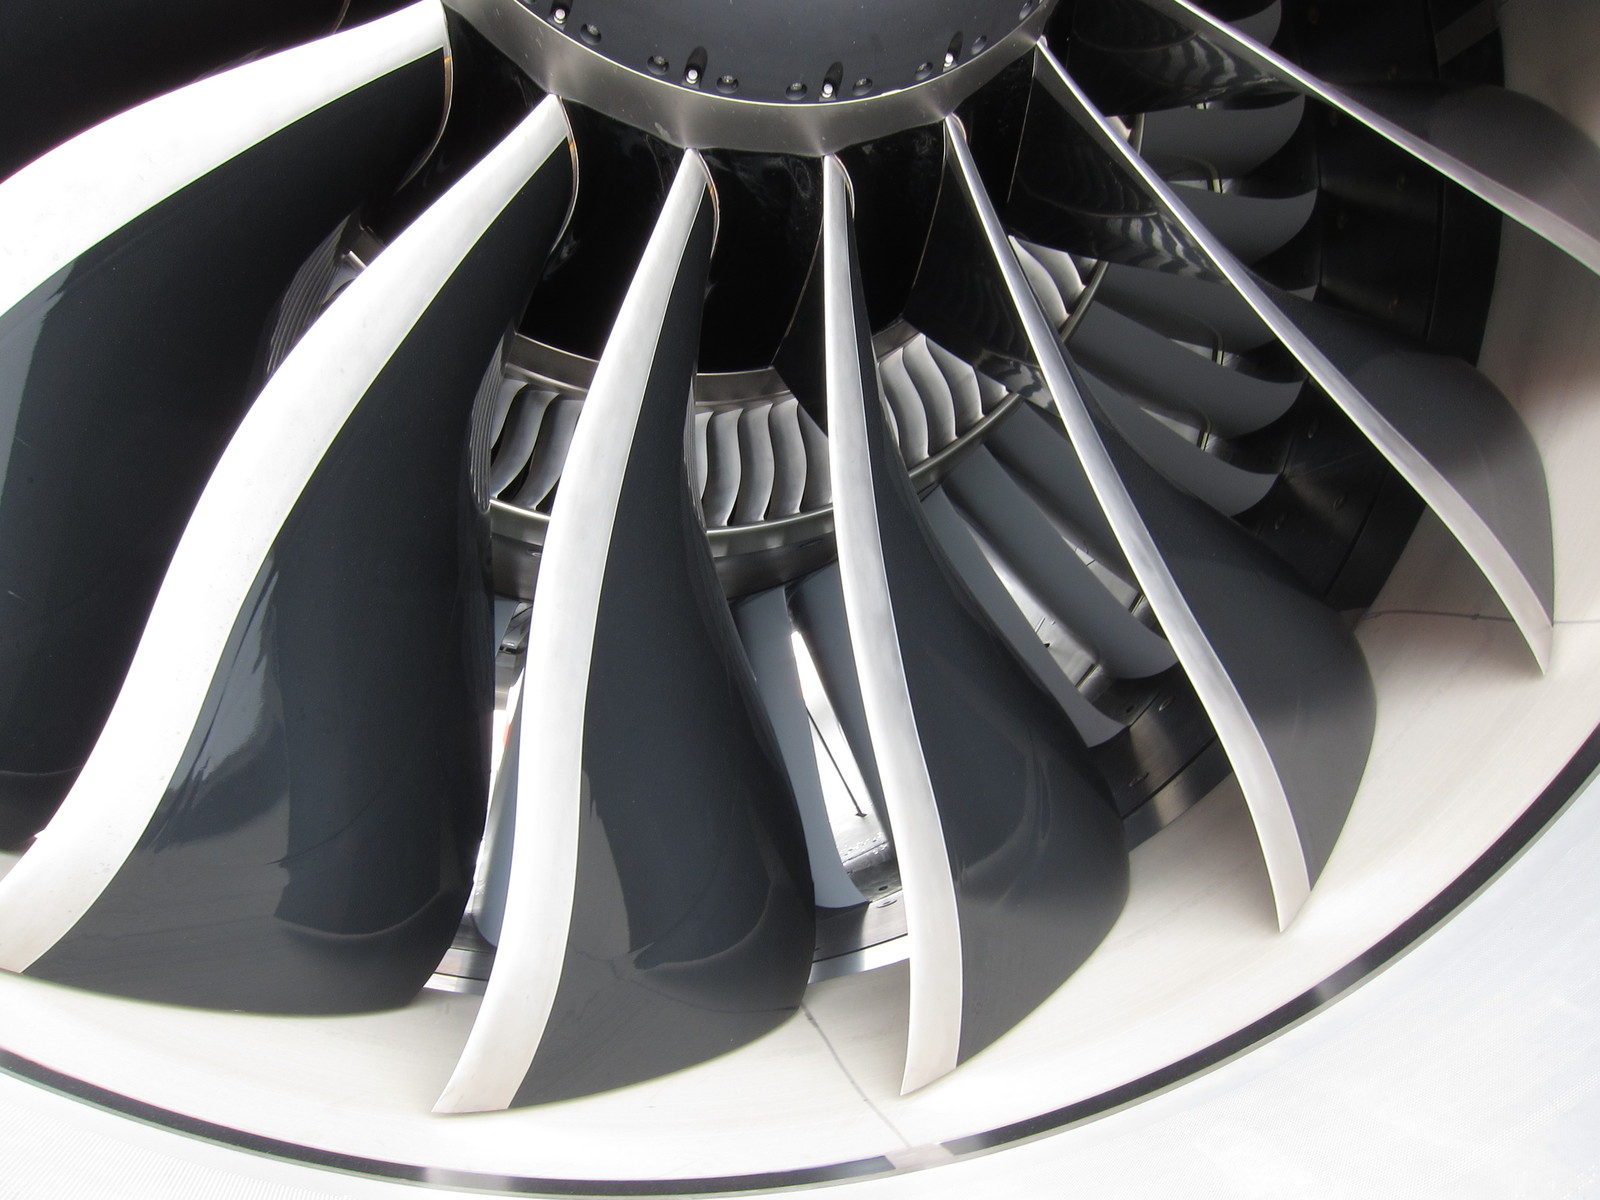
\includegraphics[width=0.8\textwidth]{images/entree_genx2b.jpg}
		\end{center}
		\supercaption{Entrée d’air d’un des quatre turboréacteurs General Electric \textsc{GEnx}-2B équipant un Boeing 747-8. Les pales bicolores de la soufflante sont visibles au premier plan ; derrière, le flux d’air est divisé entre l’entrée du compresseur (intérieur) et les stators redresseurs du flux froid (extérieur). }{Photo \ccbysa \olivier}
		\label{fig_exo_entree_genx2b}
	\end{figure}

	Pendant la croisière (atmosphère : \SI{33 000}{ft} ; \SI{-50}{\degreeCelsius} ; \SI{0,25}{\bar}), le compresseur est entraîné par la turbine par le biais d’un arbre mécanique. Il reçoit~\SI{55}{\kilogram\per\second} d’air aux conditions atmosphériques, qu’il compresse jusqu’à une pression de~\SI{8}{\bar}.
	% débit de masse : 1 Trent 500 au décollage = 1000 kg/s (source "the Jet Engine" Rolls-Royce plc 2005), estimé moitié moins en croisière soit 500 kg/s. Avec taux de dillution de 9 (pour le GEnx-2B en photo) on obtient ~ 55 kg/s.
	
	\begin{enumerate}
		\item À partir de la relation suivante,
			\begin{equation}
				\left( \frac{p_1}{p_2} \right)	= \left( \frac{v_2}{v_1} \right)^{\gamma} \tag{\ref{eq_isentropique_horrible3}}
			\end{equation}
			valable pour une évolution adiabatique réversible d’un gaz parfait, montrez (sans utiliser l’\cref{eq_isentropique_horrible1}) que :			
			\begin{equation}
				\left( \frac{T_1}{T_2} \right)	=  \left( \frac{p_1}{p_2} \right)^{\frac{\gamma -1}{\gamma}}  \tag{\ref{eq_isentropique_horrible2}}
			\end{equation}
		\item Quelle est la puissance minimale théorique à fournir au compresseur ?
		\item À quelles conditions obtiendrait-on cette puissance ?
	\end{enumerate}
	
	En réalité, le compresseur demande une puissance sensiblement plus grande pour fonctionner. Nous modélisons l’évolution réelle au sein du compresseur par deux phases distinctes :

	\begin{itemize}
		\item Un réchauffement à pression constante, effectué par frottement, avec une puissance représentant~\SI{15}{\percent} de la puissance mécanique théorique calculée plus haut ;
		\item Puis, une compression idéale jusqu’à~\SI{8}{\bar}.
	\end{itemize}
	
	\begin{enumerate}
		\shift{3}
		\item Comparez la compression théorique de la question 2 et cette nouvelle évolution sur un diagramme pression-volume. Représentez-y graphiquement le travail consommé sur l’une des évolutions.
		\item Quelle est la puissance consommée par le compresseur dans ce nouveau cas de figure ?
	\end{enumerate}


\subsubsection{Compression et combustion au sein d’un moteur Diesel}
\label{exo_compression_combustion_diesel}
\wherefrom{Partiel S1 2012, 8pts}

	En 1890 un jeune ingénieur allemand épris de thermodynamique met au point un moteur de faible puissance, faible vitesse et haute efficacité dans un laboratoire (\cref{fig_exo_moteur_diesel}). Le moteur se veut robuste et simple ; il n’a qu’un cylindre. Nous étudions ici une partie de son cycle de fonctionnement. %why not more?
	
	\begin{figure}
		\begin{center}
			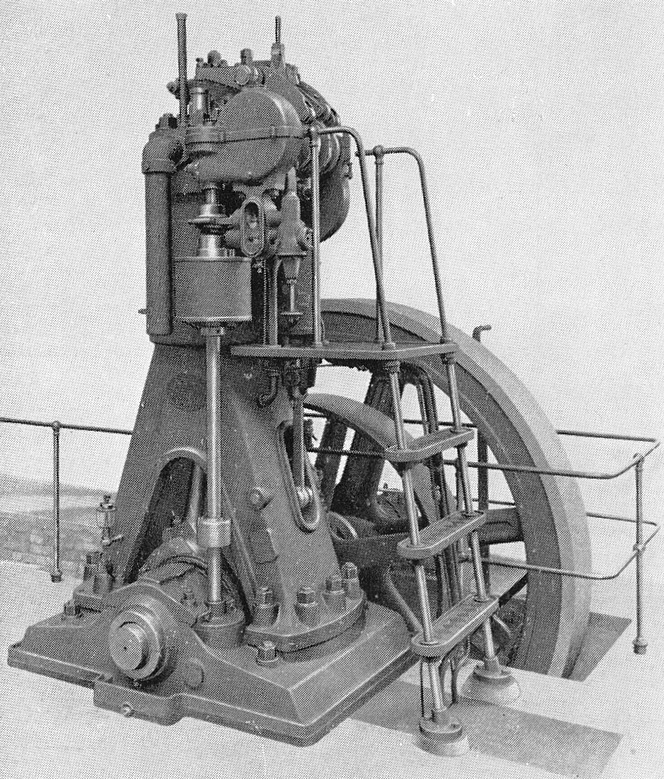
\includegraphics[width=0.5\textwidth]{images/Dieselmotor_1898_retouched.jpg}
		\end{center}
		\supercaption{Moteur Diesel de 1898, fabriqué sous licence par Sulzer en Suisse}{\wcfile{Dieselmotor 1898 (retouched).jpg}{Photo} \ccbysa Sulzer AG}
		\label{fig_exo_moteur_diesel}
	\end{figure}
	
	Le piston au sein du cylindre fait varier périodiquement le volume entre~\SI{3}{\liter} (\vocab{point mort bas}, piston en bas de sa course) et~\SI{0,3}{\liter} (\vocab{point mort haut}, piston en haut de sa course).
	
	Le moteur débute son cycle au point mort bas, alors qu’il est empli d’air à~\SI{20}{\degreeCelsius} et~\SI{1}{\bar}. Le piston comprime cet air jusqu’au point mort haut.
	
	La compression se fait de façon réversible (très lente), mais non-adiabatique : l’air reçoit de la chaleur au travers des parois tout au long de l’évolution. L’ingénieur prédit que ses propriétés varieront selon la relation $p \ v^{1,5} = \text{constante}$.


	\begin{enumerate}
		\item Le travail effectué par une force $\vec F$ sur un déplacement $\vec l$ s’exprime selon
			\begin{equation}
				W \equiv \vec F \cdot \vec l 	\tag{\ref{eq_travail_fdl}}
			\end{equation}
			À partir de cette équation, exprimez le travail effectué sur un corps de masse fixe en fonction de son volume spécifique et de sa pression interne.
		\item Combien d’énergie sous forme de travail la compression du gaz aura-t-elle coûté ?
		\item Combien d’énergie sous forme de chaleur le gaz aura-t-il reçu pendant la compression ?
	\end{enumerate}

	Lorsque le piston est arrivé en haut de sa course, on procède à l’injection progressive de carburant dans le cylindre pour permettre la combustion. La quantité de carburant injectée permet un apport total de chaleur de~\SI{2}{\kilo\joule}. La combustion se déroule à pression constante.
	
	\begin{enumerate}
		\shift{3}
		\item Représentez l’évolution suivie par le gaz pendant la compression et la combustion sur un diagramme pression-volume, de façon qualitative (c’est-à-dire sans représenter les valeurs numériques).
		\item Quelle sera la température maximale atteinte au sein du moteur ?
		\item Pour éviter une défaillance structurelle, l’ingénieur doit s’assurer que la force transmise par le piston n’excède jamais~\SI{10}{\kilo\newton}. Quelle contrainte doit-il respecter pour cela ?
	\end{enumerate}
	

\subsubsection{Turboréacteur simple flux}
\label{exo_turboreacteur_simple_flux}
\wherefrom{Partiel S1 2013, 10pts}

	Un avion militaire des années 1960 est équipé d’un turboréacteur simple flux (\cref{fig_exo_turbojet}). Nous souhaitons calculer la vitesse maximale théorique à laquelle il pourrait accélérer l’air en sortie de tuyère.
	
	\begin{figure}
		\begin{center}
			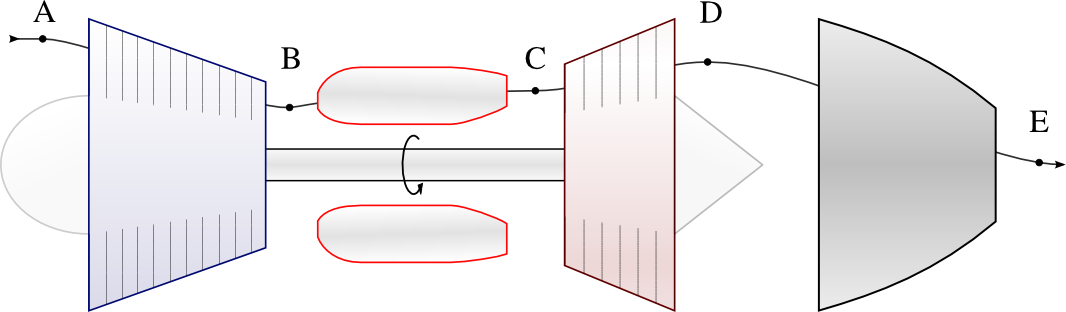
\includegraphics[width=\textwidth]{images/turbojet.png}
		\end{center}
		\supercaption{Schéma de principe d’un turboréacteur. L’air traverse la machine de gauche à droite.}{\ccbysa \olivier}
		\label{fig_exo_turbojet}
	\end{figure}
	
	Le moteur est testé sur un banc d’essai, à l’immobile. Lorsque l’air passe dans le turboréacteur, il traverse quatre composants que nous modéliserons comme s’ils étaient idéaux :
	
	\begin{description}
		\item [Le compresseur] (\cref{fig_exo_compresseur_turbojet}) comprime l’air de façon adiabatique réversible.\\
			À l’entrée, l’air est à~\SI{0,9}{\bar} et~\SI{5}{\degreeCelsius} ; à la sortie la pression est portée à~\SI{19}{\bar}.
		\item [La chambre de combustion] permet d’effectuer un réchauffement de l’air en maintenant sa pression constante.\\
			À la sortie de la chambre de combustion, la température a été portée à~\SI{1100}{\degreeCelsius}.
		\item [La turbine] extrait de l’énergie de l’air pour pouvoir alimenter le compresseur. Dans la turbine, l’air est détendu de façon adiabatique réversible.
		\item [La tuyère] est un composant dans lequel aucune puissance n’est apportée ni prélevée à l’air. Lorsqu’il la traverse, l’air se détend de façon adiabatique réversible ; sa vitesse augmente fortement. À la sortie de la tuyère, il a retrouvé la pression atmosphérique et est rejeté dans l’atmosphère.
	\end{description}
	
	Le but de l’exercice est de calculer la vitesse à laquelle le turboréacteur est capable de repousser l’air qu’il admet.
	
	\pagebreak[1] %handmade
	
	\begin{enumerate}
		\item À partir de la relation suivante,
			\begin{equation*}
				\left( \frac{T_1}{T_2} \right)	= \left( \frac{v_2}{v_1} \right)^{\gamma -1}
			\end{equation*}
			valable pour une évolution adiabatique réversible d’un gaz parfait, montrez (sans utiliser l’équation~\ref{eq_isentropique_horrible3}) que :			
			\begin{equation*}
				\left( \frac{T_1}{T_2} \right)	=  \left( \frac{p_1}{p_2} \right)^{\frac{\gamma -1}{\gamma}}
			\end{equation*}
		\item Quelle est la température de l’air à la sortie du compresseur ?
		\item Quelle est ainsi la puissance spécifique consommée par le compresseur ?
		\item Quelle est la puissance spécifique apportée sous forme de chaleur dans la chambre de combustion ?
		\item Quelle doit être la température à la sortie de la turbine pour qu’elle puisse alimenter le compresseur ?
		\item Quelle sera alors la pression à la sortie de la turbine ?
		\item Quelle sera la température des gaz d’échappement, à la sortie de la tuyère ?
		\item Quelle sera enfin la vitesse d’éjection des gaz à la sortie de la tuyère ?
		\item Représentez l’évolution sur un diagramme pression-volume, de façon qualitative.
		\item Sur le même diagramme pression-volume, tracez l’évolution qui serait suivie par le gaz si le compresseur ne pouvait pas effectuer une compression réversible (compresseur réel, compression avec frottement interne).
	\end{enumerate}

	
	\begin{figure}[bth]
		\begin{center}
			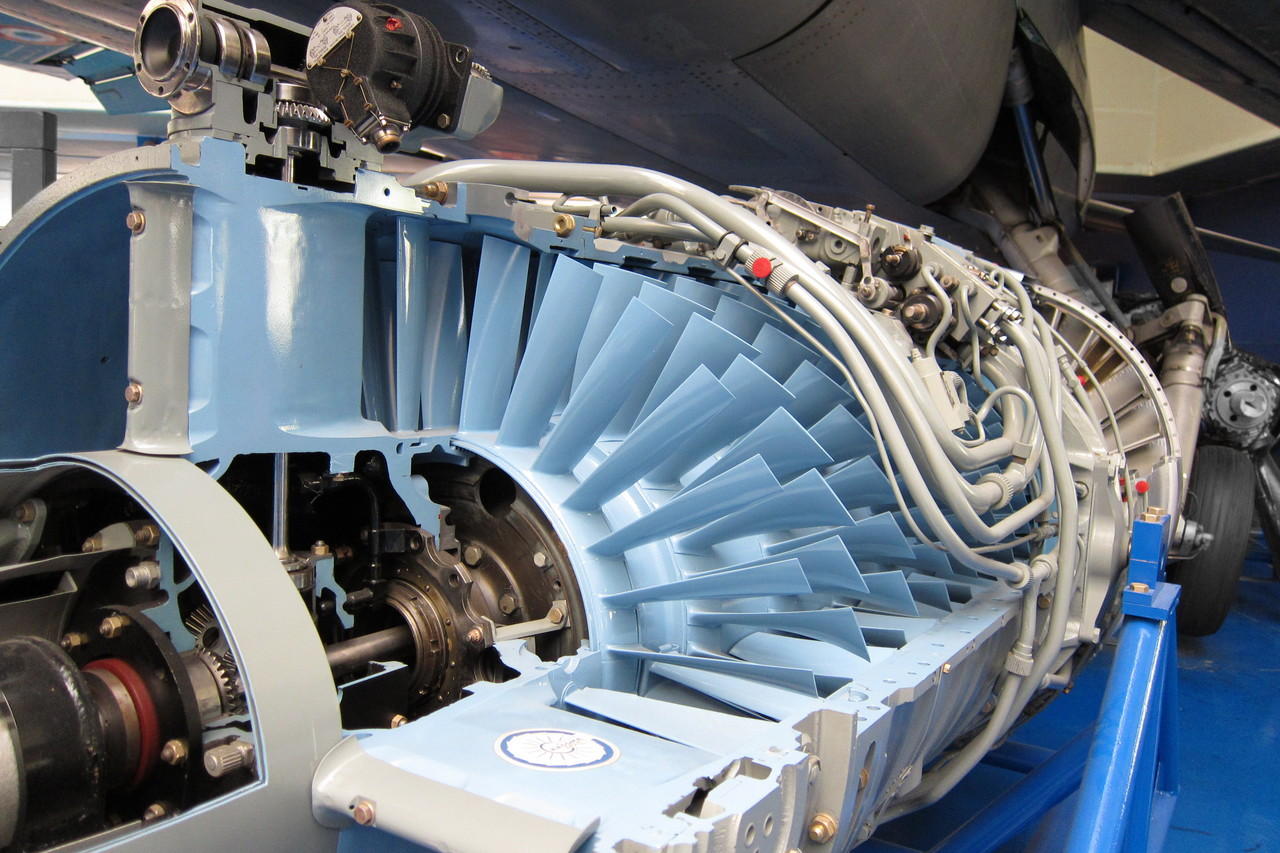
\includegraphics[width=0.8\textwidth]{images/atar_compressor.jpg}
		\end{center}
		\supercaption{Compresseur d’un turboréacteur simple flux \wfd{Snecma Atar}{\textsc{snecma} Atar} (1948) découpé. L’air s’écoule depuis le coin gauche vers le centre de l’image.}{\wcfile{Compressor of Atar turbojet.jpg}{Photo} \ccbysa \olivier}
		\label{fig_exo_compresseur_turbojet}
	\end{figure}


\exercisesolutionpage
\titreresultats

\begin{description}
	\item [\ref{exo_pression_air}]
					\tab 1) $v_1 = \frac{V_1}{m_1} = \SI{0,4}{\metre\cubed\per\kilogram}$ ; $\rho_1 = \frac{1}{v_1} = \SI{2,5}{\kilogram\per\metre\cubed}$
					\tab 2) $p_1 = \frac{R T_1}{v_1} = \SI{2,103}{\bar}$.
	\item [\ref{exo_rechauffement_reservoir_air}]
					\tab 1) $m_1 = \frac{p_1 V_1}{R T_1} = \SI{3,006}{\kilogram}$ ; $v_1 = \SI{0,3991}{\metre\cubed\per\kilogram}$ ; $\rho_1 = \SI{2,505}{\kilogram\per\metre\cubed}$ ; $p_1 = \SI{2}{\bar}$ ;
					\tab ~~ $m_2 = m_1$ ; $v_1 = v_2$ ; $\rho_1 = \rho_2$ ; $p_2 = \frac{R T_2}{v_2} = \SI{2,395}{\bar}$.\\
					\tab 2) $m_3 = \SI{2,51}{\kilogram}$, ainsi $m_\text{échap.} = m_3 - m_2 \SI{0,4959}{\kilogram}$ ;
					\tab 3) $p_4 = \frac{R T_4 m_4}{V_4} = \SI{1,67}{\bar}$.
	\item [\ref{exo_gp_energie_temperature}]
					\tab $\Delta u = c_v T_3 - u_1 = \SI{-536}{\kilo\joule\per\kilogram}$ (se calcule simplement avec la température finale et ne dépend pas de l’évolution ou des états intermédiaires).
	\item [\ref{exo_puissance_pompe_air}]
					\tab $w_{1\to 2} = \Delta h = c_p \Delta T = \SI{+85,4}{\kilo\joule\per\kilogram}$ (\ref{eq_petite_sfee_deltas_h} \& \ref{eq_h_fonction_de_T})
	\item [\ref{exo_gp_turbine_turboreacteur}]
					\tab 1) Avec l’\cref{eq_petite_sfee_deltas_h}, $w_\text{turbine} = c_p (T_\B - T_\A) + \frac{1}{2}(C_\B^2 - C_\A^2) - q_\fromatob = \SI{-275}{\kilo\joule\per\kilogram}$ 	
					\tab 2) $\dot m = \frac{\dot W_\text{turbine}}{w_\text{turbine}} = \SI{3,64}{\kilogram\per\second}$
	\item [\ref{exo_gp_isotherme}]
					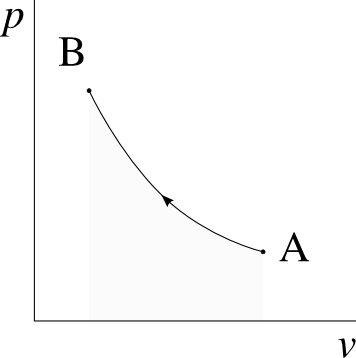
\includegraphics[width=\solutiondiagramwidth]{images/exo_sol_pv_isoth.png}
					\tab 2) Avec l’\cref{eq_gp_travail_isotherme_sf1}, $w_{1 \to 2} = \SI{+257,58}{\kilo\joule\per\kilogram}$ (donc un travail reçu) ; $W_{1 \to 2} = \SI{+901,2}{\kilo\joule}$ ; $Q_{1 \to 2} = - W_{1 \to 2}$ (donc une dépense de chaleur)\\
				 	\tab 3) Oui, on aurait $v_{2 \text{ad.rév.}} = v_1 \left(\frac{p_1}{p_2}\right)^{\frac{1}{\gamma}} > v_{2 \text{isoth.}} =  v_1 \left(\frac{p_1}{p_2}\right)$.
	\item [\ref{exo_gp_isobare_isochore}]
					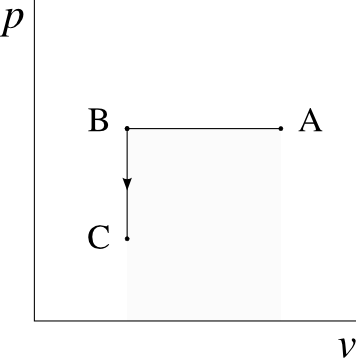
\includegraphics[width=\solutiondiagramwidth]{images/exo_sol_pv_isob_isoch.png}
					\tab 2) $W_{1 \to 3} = -\int_1^2 p \diff V - \int_2^3 p \diff V = -p_\text{cste} \Delta V - 0 = \SI{+153,6}{\kilo\joule}$	
					\tab 3) $Q_{1 \to 3} = U_3 - U_1 - W_{1 \to 3} = m c_v \left(T_3 - \frac{p_1 V_1}{m R}\right) - W_{1 \to 3} = \SI{-625,3}{\kilo\joule}$
	\item [\ref{exo_gp_isentropique}]
					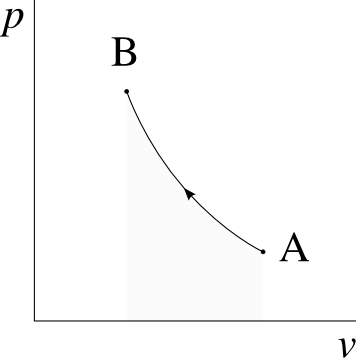
\includegraphics[width=\solutiondiagramwidth]{images/exo_sol_pv_isentr.png}
						\tab Cas optimal : compression adiabatique réversible. Avec l’équation~\ref{eq_isentropique_horrible2}, on calcule $T_\B = \SI{896,4}{\kelvin}$ ; $W_\text{minimal} = m \ c_v (T_\B - T_\A) = \SI{+2,157}{\mega\joule}$.
	\item [\ref{exo_bete_mechant}]
						\tab Isotherme $2 \to 3$, isochore $1 \to 2$.
	\item [\ref{exo_retrouver_pv}]
						\tab \textit{Dans le sens horaire, en débutant à l’horizontale, sur les deux graphiques :} isobare ($p$~cste.), isotherme ($T$~cste.), adiabatique réversible, isochore ($v$~cst.).
	\item [\ref{exo_compresseur_turboreacteur}]
						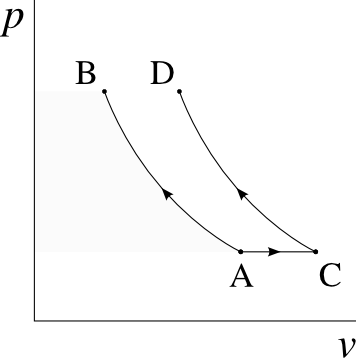
\includegraphics[width=\solutiondiagramwidth]{images/exo_sol_pv_turbojet_compressor.png}
						\tab 1) Remplacer $v_2$ par $\frac{R T_2}{p_2}$, faire de même avec $v_1$. Dérouiller son algèbre et le résultat vient tout seul ;
						\tab 2) Avec l’équation~\ref{eq_isentropique_horrible2}, on obtient $T_\B = \SI{600,7}{\kelvin}$, ainsi $\dot{W}_{\fromatob} = \SI{+20,87}{\mega\watt}$ ;
						\tab 3) \S\ref{ch_gp_isentropiques} ;
						\tab 5) $T_\C = \SI{279,8}{\kelvin}$ ; $T_\D = \SI{753,1}{\kelvin}$ ; Ainsi $\dot{W}_\text{compresseur réel} = \dot{W}_{\text{pertes frottement} \A \to \C} + \dot{W}_\fromctod = \SI{+29,29}{\mega\watt}$ (\SI{+40}{\percent}).
	\item [\ref{exo_compression_combustion_diesel}]
						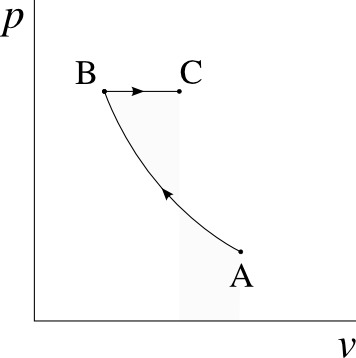
\includegraphics[width=\solutiondiagramwidth]{images/exo_sol_pv_diesel.png}
						\tab 1) voir \S\ref{ch_travail_pdv} \& \S\ref{ch_travail_fdl}
					 	\tab 2) $W_{\fromatob} = - m \int_\A^\B p \diff v = \SI{+1,298}{\kilo\joule}$ 	
						\tab 3) Avec $p_\B = k v_\B^{\num{-1,5}} = \SI{31,6}{\bar}$, on a $T_\B = \SI{926,3}{\kelvin}$. Enfin, $Q_{\fromatob} = \Delta U - W_{\fromatob} = \SI{+0,3254}{\kilo\joule}$.
						\tab 5) À pression constante, avec l’\cref{eq_q_gp_sf_isobare},  $T_\C = \frac{Q_\frombtoc}{m \ c_p} + T_\B = \SI{1483,7}{\kelvin}$ (\SI{1211}{\degreeCelsius}).
						\tab 6) $S < \frac{F_\text{max.}}{p_\C} = \SI{3,164e-3}{\metre\squared}$ (diamètre $D_\text{max} = \SI{6,35}{\centi\metre}$).
	\item [\ref{exo_turboreacteur_simple_flux}]
						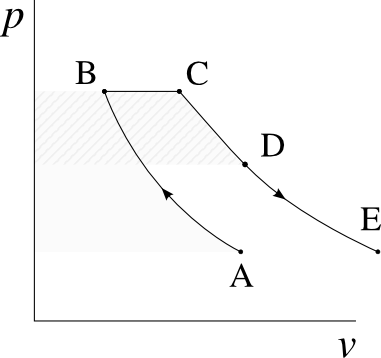
\includegraphics[width=\solutiondiagramwidth]{images/exo_sol_pv_turbojet_1.png}
						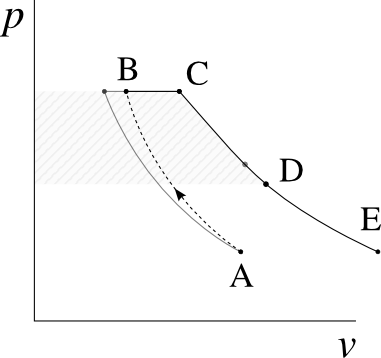
\includegraphics[width=\solutiondiagramwidth]{images/exo_sol_pv_turbojet_2.png}
						\tab 2) Avec l’équation~\ref{eq_isentropique_horrible2}, $T_\B = \SI{664,83}{\kelvin}$
						\tab 3) Avec l’\cref{eq_petite_sfee_deltas_h}, $w_\text{compresseur} = w_\fromatob = \SI{+338,61}{\kilo\joule\per\kilogram}$
						\tab 4) $T_\C = \SI{1373,15}{\kelvin}$ ; ainsi $q_\text{combustion} = q_\frombtoc = \SI{+711,86}{\kilo\joule\per\kilogram}$
						\tab 5) Comme $w_\text{turbine} = - w_\text{compresseur}$, on a $T_D = \SI{986,47}{\kelvin}$
						\tab 6) Avec l’équation~\ref{eq_isentropique_horrible2}, $p_\D = \SI{5,97}{\bar}$
						\tab 7) Idem, avec l’équation~\ref{eq_isentropique_horrible2}, $T_\text{E} = \SI{574,49}{\kelvin}$
						\tab 8) Avec l’\cref{eq_petite_sfee_deltas_h}, $C_\text{E} = \left(-2\Delta h\right)^\frac{1}{2} = \SI{909,98}{\metre\per\second}$\\
						\tab Bien sûr, ces valeurs ne tiennent pas compte des irréversibilités existant dans un turboréacteur réel. Ces effets sont abordés dans l’exercice \ref{exo_compresseur_turboreacteur} et formalisés dans le \coursdix.
\end{description}
